%%%%%%%%%%%%%%%%%%%%%%%%%%%%%%%%%%%%%%%%%%%%%%%%%%%%%%%%%%%%%%%%%%%%%%%%%%%%%%%%
%2345678901234567890123456789012345678901234567890123456789012345678901234567890
%        1         2         3         4         5         6         7         8

\documentclass[letterpaper, 10 pt, conference]{ieeeconf}  % Comment this line out if you need a4paper

%\documentclass[a4paper, 10pt, conference]{ieeeconf}      % Use this line for a4 paper

\IEEEoverridecommandlockouts                              % This command is only needed if 
                                                          % you want to use the \thanks command

\overrideIEEEmargins                                      % Needed to meet printer requirements.

%In case you encounter the following error:
%Error 1010 The PDF file may be corrupt (unable to open PDF file) OR
%Error 1000 An error occurred while parsing a contents stream. Unable to analyze the PDF file.
%This is a known problem with pdfLaTeX conversion filter. The file cannot be opened with acrobat reader
%Please use one of the alternatives below to circumvent this error by uncommenting one or the other
%\pdfobjcompresslevel=0
%\pdfminorversion=4

% See the \addtolength command later in the file to balance the column lengths
% on the last page of the document

% The following packages can be found on http:\\www.ctan.org
%\usepackage{graphics} % for pdf, bitmapped graphics files
%\usepackage{epsfig} % for postscript graphics files
%\usepackage{mathptmx} % assumes new font selection scheme installed
%\usepackage{times} % assumes new font selection scheme installed
%\usepackage{amsmath} % assumes amsmath package installed
%\usepackage{amssymb}  % assumes amsmath package installed
\usepackage{graphicx}
\graphicspath{ {./images/} }
\usepackage{subcaption}
\usepackage{url}
\usepackage{booktabs}
\usepackage{hyperref}

\title{\LARGE \bf
Using Scene Graph Generation to Support LLM-Based Queries to a Vision System}


\author{Raghav Rangan, Siddh Bamb, Kevin Zhao, Zhongyan He% <-this % stops a space
}
%\thanks{*This work was supported by...}% <-this % stops a space
%\thanks{$^{1}$Christina Petlowany is with the Cockrell School of Engineering,
%        The University of Texas at Austin, Austin, TX 78712, USA
%        {\tt\small cpetlowany@utexas.edu}}%
%\thanks{$^{2}$Justin Hart is with the College of Natural Sciences, The %University of Texas at Austin,
%        Austin, TX 78712, USA
%        {\tt\small justinhart@utexas.edu}}%
%}

% todo other authors


\begin{document}



\maketitle
\thispagestyle{empty}
\pagestyle{empty}


%%%%%%%%%%%%%%%%%%%%%%%%%%%%%%%%%%%%%%%%%%%%%%%%%%%%%%%%%%%%%%%%%%%%%%%%%%%%%%%%
\begin{abstract}
    The purpose of our project is to design and implement an LLM-based system to take a query regarding the internal state of a mapped space and answer it using labeled map data. Our goal is to make a robotic system capable of relating objects to each other both semantically and positionally in order to make it possible for it to answer questions or simply describe with relevant detail the space it has mapped. We propose a system that creates map data through the use of a scene graph generation (SGG) model. The output of this model, which is a relational graph connecting all the objects the network detects in the scene, is converted into a set of descriptive phrases using a simple algorithm, and fed into GPT-3.5, which handles the querying process. Our results showed that ChatGPT is very good at answering questions based on information previously provided to it, and our SGG model was able to create a detailed and accurate enough relational graph of several test scenarios to make the entire system operate functionally.
\end{abstract}
    
\section{Introduction}
    We began our project with an investigation into existing object detection frameworks, namely CLIP, to test how accurately it could identify relational phrases in an input image. We found that it did quite poorly, often detecting contradictory phrases with equal confidence. Our focus shifted onto finding a better way to handle object detection, and we decided on scene graph generation. In essence, an SGG model is capable of taking an input image, detecting objects within it, and creating a graph that relates each of the objects with another. The vertices of this graph are the objects, and the edges connecting them are the relationship. We chose an SGG model trained on Visual Genome \cite{Krishna_Zhu_Groth_Johnson_Hata_Kravitz_Chen_Kalantidis_Li_Shamma_et_al._2017}, a dataset containing various images annotated with a relational graph of their contents. In this way, the edges of our output graph would be prepositions, thus drawing a positional relationship between a pair of objects. Turning the resultant graph into a set of phrases is accomplished by iterating through the pairs and adding them to a string. We feed this body of text into ChatGPT through the GPT-3.5 API. Specifically, we prompt ChatGPT to answer the following questions based on a body of text, and then provide it with our output paragraph. Finally, the end user is able to interact with the data, asking questions like, "How many chairs are in the room?", "Is there a lamp next to the couch?", etc.

\section{Related Works}
    As part of our preliminary research, we looked into how CLIP, CLIPSeg \cite{lueddecke22_cvpr}, and joint embedding spaces work. CLIP is a contrastive learning image model that takes advantage of a joint embedding space mapped onto by both a text encoder and image encoder \cite{radford2021learning}. By training the encoders to map semantically similar text and images to similar values and push away dissimilar ones, the model can then pick what text matches the image most accurately. This allows for impressive zero shot performance, much better than previous models like ImageNet. We initially provided the CLIP model with a list of relationships we wanted it to find in an input image, such as "Person next to table", "Laptop on table", etc. What we found was that CLIP performs poorly when trying to infer positional relationships between objects in the frame. Furthermore, descriptions where one object was present in the picture and the other wasn't created inconsistent outputs from the CLIP model.

    However, when we fed a paragraph of CLIP's top-20 outputs to ChatGPT, we found that the LLM interface was very good at remembering a set of information and answering queries regarding that information correctly. In other words, it was correctly identifying details from the input paragraph, and providing answers that were consistent with the body of information we provided. This initial experiment proved the need for an alternative method to identify positional relationships between objects, and proved the viability of ChatGPT as a functional LLM interface to answer queries given a body of information.

    From these findings, we explored alternative techniques to identify inter-object relationships, and we decided to proceed with scene graph generation (SGG). An SGG model is capable of generating a graph given an image, such that nodes in this graph reperesent objects detected, and edges represent the positional relationship between the vertices they connect. We decided to pursue this technique after encountering the Visual Genome dataset. Our exploration began with the Graph-RCNN network \cite{yang2018graph}, a model that builds on top of the Faster-RCNN object detection framework to allow for scene graph generation. Specifically, the model uses a novel combination of a Relational Proposal Network, which handles predicting object relatedness, and a Graph Convolutional Network, which procedurally generates the output graph based on the object relations predicted by the RePN. The output is a refined, pruned graph, containing objects and their relevant relations. However, we continued to look into more modern SGG techniques, and discovered Neural Motifs \cite{zellers2018scenegraphs}, a paper that explored a different approach to SGG, focused on the fact that inter-object relations have a very repetitive nature, often remaining the same between identical objects in different scenes. The introduction of this idea allows for the model to predict these patterns or motifs across images, often correctly predicting edges that did not exist in provided ground-truth test images. We then looked into the current state-of-the-art, and found a model, Causal-TDE, to have the highest recall@50 on the Visual Genome dataset \cite{latestinML}. This model tries to solve one of the main issues in SGG, which is training bias. Due to more generic relations being more common in datasets, SGG models tend to predict more generic relations between things when they actually have the information to provide a more specific relation. For example, "Person riding on bike" vs. "Person on bike" \cite{tang2020unbiased}. To counter this, the model makes two inferences, one considering the two objects (biased), and one with the two objects removed from the image (unbiased). Taking the difference in the predicted relation vectors between the two inferences, also known as Total Direct Effect (TDE) provides a more accurate and detailed relation between the objects \cite{tang2020unbiased}. The actual graph generation done by this model is handled by a MotifNet \cite{zellers2018scenegraphs}, but it is made to generate a causal graph and a counterfactual graph, the difference of which is taken as a final prediction. 



\section{Methodology}
    Our final system will take the form of a pipeline having three stages:
    \begin{itemize}
        \item The SGG model
        \item Phrase Generation to convert output JSON into a context string
        \item ChatGPT interface to answer queries with information from the set of phrases.
    \end{itemize}

    \subsection*{The SGG Model}
        For this project we use a pre-trained SGG Model, trained on the Visual Genome dataset. The model is capable of generating a well-connected graph of relationships between objects. This is achieved through two stages, an object detection stage, and the graph generation stage. The object detection stage creates bounding boxes around all detectable objects in the input image. The bounding boxes are calculated around each object, refined, and then stored to keep track of the relative positions of each object in the scene. At this point, the data is passed to the graph generation stage.
        The Visual Genome dataset splits the graph of each image into two classes: objects (nouns, such as "car", "person", etc.) and predicates (prepositions or verbs, such as "on top of", "riding on", etc.).
        
        The generated graph's vertices represent objects, while the directed edges connecting them represent the predicate, or relationship between the source vertex and destination vertex. The specific pre-trained model we use is from Causal-TDE \cite{tang2020sggcode}, which is a state-of-the-art SGG model, using a VGG-based RCNN object detection backbone, and a custom graph generation architecture to achieve higher recall results than previous SGG models. The key differentiating factor is that the final prediction is a result of the difference between a calculated causal graph and a counterfactual graph, which eliminates some training bias that generifies the output relation in previous models. An example of a TDE calculation and its effect on the output prediction is shown in Figure 2.

        \begin{figure}
            \centering
            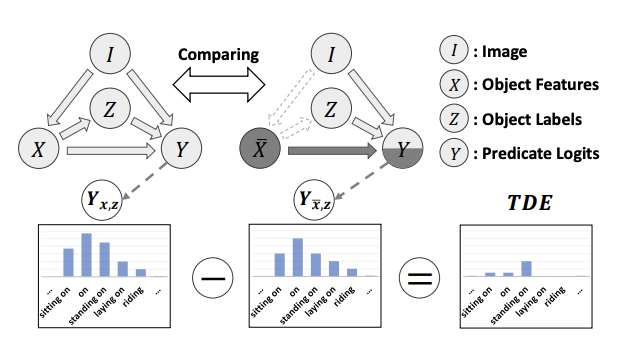
\includegraphics[width=0.4\textwidth]{images/counterfactual.png}
            \caption{Total Direct Effect calculation showing how the difference between the causal and counterfactual graphs result in a more detailed final prediction. (used from Tang et. al. \cite{tang2020unbiased}). The column with the greatest change (the largest difference) is the predicate whose prediction changed the most across the two graphs, making it a feature of interest that would not be predicted with a single inference, but is predicted when TDE is calculated.}
            \label{fig:counterfactual}
        \end{figure}


    
    \subsection*{Phrase Generation}
        Since the output of the model is a JSON file, containing a list in the format \{object, relation, object\}, we need an algorithm that can turn the list into a large string describing the entire set of relatiomships. We go through the output list from the SGG model, and turn each of the entries from the JSON file into a string of the form (object =\textgreater  relation =\textgreater  object). Furthermore, our tests with the ChatGPT interface showed that the LLM is able to accurately and consistently describe a space given the limited description we showed above. We further optimized the phrase generation to account for duplicate objects. While the object detection layer of the SGG model indexes its labels to differentiate duplicate objects, passing the labels directly to the GPT interface is not ideal, since duplicate labels look like "couch2" or "lamp4". We instead look at the label's position in the triplet and label it appropriately. For example, "couch2 right of lamp" would be converted to "second couch right of lamp", allowing GPT to not confuse "couch2" for some unknown object while still maintaining the difference between the couches found in the image.
    
    \subsection*{ChatGPT Interface}
        The final stage of the pipeline is the ChatGPT Interface, which supports the main purpose of our system: relational queries. Using our lab's GPT API key, we were able to interact directly with ChatGPT from our code. However, we needed to provide the information generated by the phrase generation in a customized query, so that the LLM is prepared to answer any following questions based on its original body of information. However, an important consideration for us was that people could provide the model with new information, overriding the original body of text we provided to it. We provide the body of information regarding the room to the API as a context string, which is immutable from the side of the user, ensuring that the interface's information base is never changed. The query is passed into a function containing the context, which then creates a response by passing the query and the context to the API. In this way, we are able to get consistent and meaningful output from the ChatGPT interface, and ensure that the context is never tampered with.


\section{Experimental Setup}
\subsection*{Training}
    Since we used a pre-trained model, we do not have to consider training techniques, or preprocessing data from Visual Genome. Rather, we are directly able to feed image inputs to our system and evaluate their accuracy in comparison to the real world.

\subsection*{Evaluation}

    Our first metric of evaluation will be accuracy. To measure this, we will be using a set of sample images, and feedign them into our system. We will then examine the output of the phrase generation stage to determine how well the objects and their relationships were detcted. We count the number of unique objects in the generated context string and compare it to the total number of objects present in the image to determine the proportion of detected objects, giving us an idea of how much of the image's detail the context string captures. We want to minimize or even entirely avoid false positives, so we will keep a count of objects that show up in the context string that are not present in the image. We want to maximize the percentage of detected objects while minimizing the false positive count, which would imply a system that extracts a lot of detail while not making mistakes. We will also maintain a false positive count for the relationships found in the context string, to ensure that no incorrect relationships are being predicted. These three numbers will provide good insight into the performance of our model from an accuracy perspective.

    Second, since our goal is to make our system's interaction feel as human as possible, our experiment will involve a practical test that evaluates the final GPT interface layer. We will have subjects interact with a human describing the space as well as our frontend, without knowing which one they are talking to. We will then ask them which they thought was which. Statistical tests can then be run on this data to see if there was a statistically signficant result (people were able to recognize which interaction was which correctly). A significant difference would mean our system is distinguishable from a human's description, which is a negative. We are looking for an insignificant result from this test, which would mean our system's output is highly similar to a real person's description.

    An important application of our system is to assist the visually impaired with perceiving a space. In other words, we want to naturally answer queries about a space in order to provide a visually impaired individual with an accurate and detailed description of a space. Therefore, the conversational aspect of the robot is second in importance after its accuracy.


\section{Results}
    We were able to successfully build and run the pre-trained Causal-TDE checkpoint on multiple sample images, and we found predictions that were accurate to the state of the scene in the image. Furthermore, the object detection stage correctly identified a variety of objects in the room, and the generated relations reflected a pruned version of the graph, containing relations between objects that were contextually and physically close to each other. A sample result can be seen in Figures 2a and 2b.

    \begin{figure}
        \centering
        \begin{subfigure}{0.48\textwidth}
            \centering
            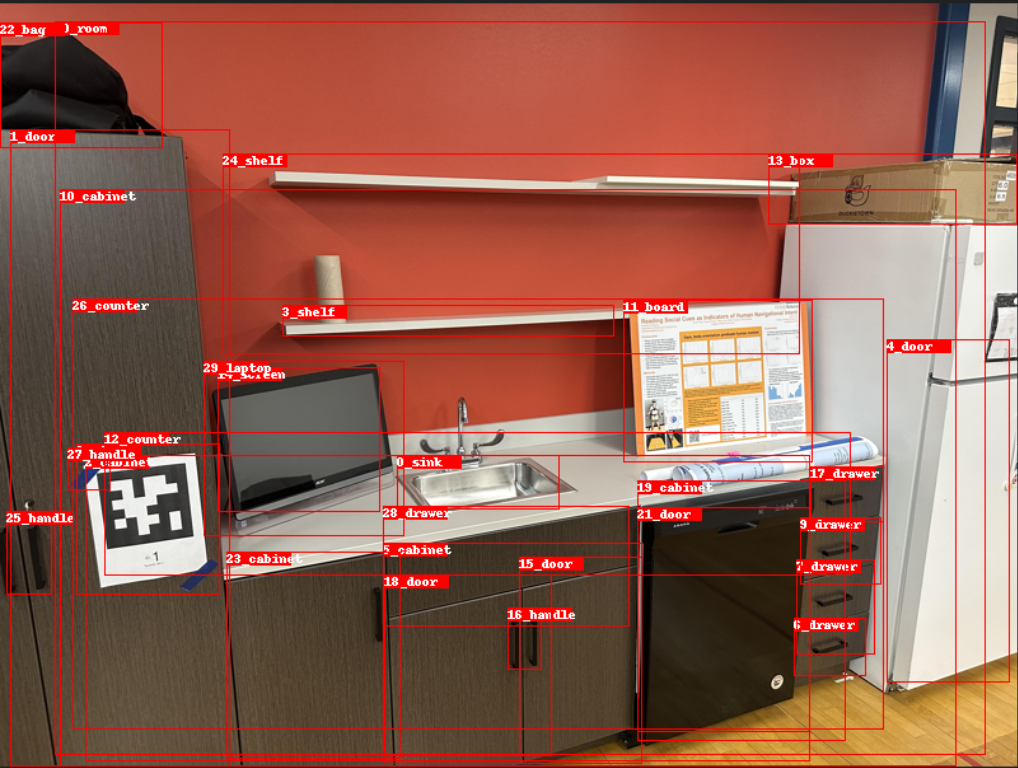
\includegraphics[width=1\textwidth]{images/scene.png}
            \caption{Output of object detection stage, shows bounding boxes around all detected objects in a sample scene of the AHG Lab.}
            \label{fig:outputs}
        \end{subfigure}
        \begin{subfigure}{0.48\textwidth}
            \centering
            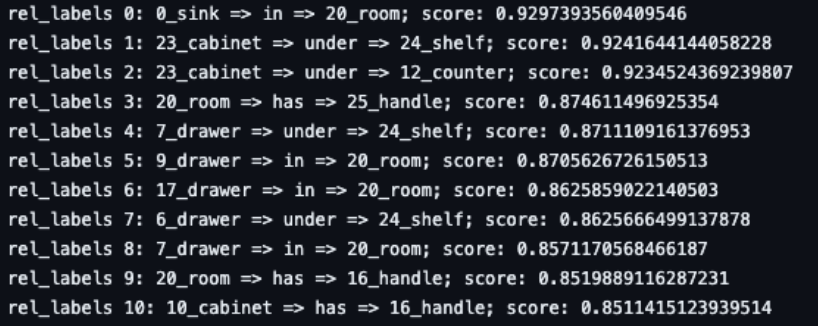
\includegraphics[width=1\textwidth]{images/graph.png}
            \caption{Output of graph generation. Shows multiple reltions between objects detected in the scene. All shown outputs are correct, and can be seen/found in the original image in Figure 2a.}
            \label{fig:graph}
        \end{subfigure}
        \begin{subfigure}{0.48\textwidth}
            \centering
            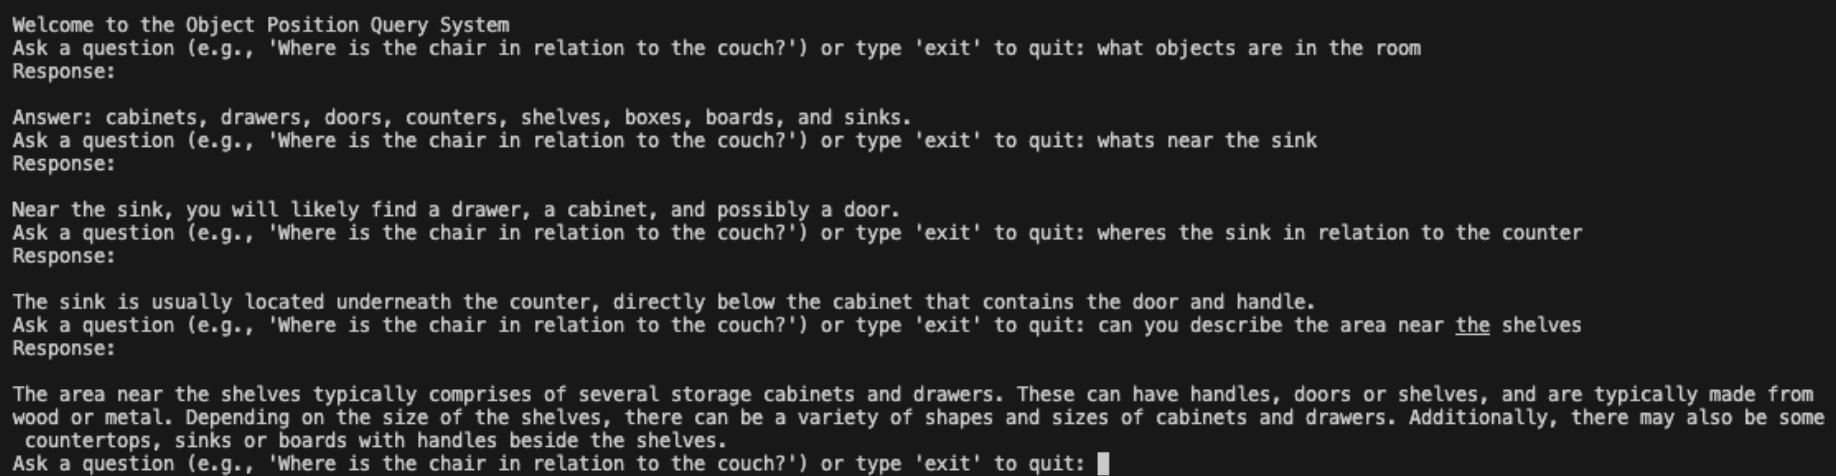
\includegraphics[width=1\textwidth]{images/output.png}
            \caption{Output of conversation with GPT. All of the responses' correctness can be verified from the original image.}
            \label{fig:output}
        \end{subfigure}
        \caption{An example output from the SGG model}
        \label{fig:example}
        
    \end{figure}

    We then tested the entire pipeline, providing the output JSON of the SGG model to the phrase generator, and running some test queries with the GPT API to see how well it was able to converse given the generated context string. We found the conversations to be detailed, natural, and, most importantly, accurate to the picture of the room. Furthermore, we also showed that malicious user input that tried to change the context was unsuccessful, since the API clearly separates input and context, allowing us control of the security of the system. An example of the output is shown in Figure 2c, and we transcribe a few responses here:
    \begin{itemize}
        \item \textit{Question:} What's near the sink? \\ \textit{Answer:} Near the sink, you will likely find a drawer, a cabinet, and possibly a door.
        \item \textit{Question:} Can you describe the area near the shelves? \\ \textit{Answer:} The area near the shelves typically comprises of several storage cabinets and drawers. These can have handles, doors or shelves, and are typically made from wood or metal. Depending on the size of the shelves, there can be a variety of shapes and sizes of cabinets and drawers. Additionally, there may also be some countertops, sinks or boards with handles beside the shelves.
    \end{itemize}

    For our accuracy measurements:
    We tested on a set of 8 sample images, and for each image, collected the top 10 and top 25 most confident outputs from the SGG model. We then counted the number of unique labels present in the output and compared this to the total number of labels detected by the object detection layer to calculate the percentage of present objects that were reflected in the SGG model's output. For the top 10 case, we found mediocre results, with an average of 49\% and a standard deviation of 6.6\%. However, upon increasing the cutoff to the top 25, our numbers improved greatly, to an average of 74.25\% and a standard deviation of 6.5\%. Our experimental data can be found in Table 1 in the Appendix. Clearly, with lower cutoffs, more of the objects will be included in the SGG model's output. However, by reducing the cutoff for the confidence, we increase the chance of redundant and/or incorrect triplets, and a next step would be to determine the optimal cutoff that balances these two things. As for the false positive count, across all 8 images we had a count of 1 for false positive objects detected, and a count of 0 for false positive triplets / relationships predicted. This is a very positive result, as it shows that our system makes very few if any incorrect predictions, meaning our area of improvement is entirely dealing with increasing the quality and quantity of detail captured.

    Finally, we measured the 'humanness' of our system's interactive capability by asking participants to compare our system's output vs. a human's for a fixed set of questions and try to determine which one was produced by our system. Our results show\dots.

\section{Discussion}
    While the results are very promising, and show that our approach is capable of successfully inferring positional relationships between objects detected in a 2D image input, we need to implement this system on a robot to verify its entire functionality. More specifically, we need to implement our pipeline using ROS nodes, and feed the robot's camera feed as image input to the SGG model.

    Furthermore, we hope to look into potential improvements to the SGG model, including upgrading its object detection framework, or optimizing the phrase generator to allow GPT to extract even more detail from our context input.

    Another long-term improvement would be to make the SGG inferences dynamic. We would want to support continuous information updates for the use case of a system that can accompany a visually impaired person on a tour or some guided interaction. We would like to support periodically updating the context string with a new set of relationships as the robot navigates a space, so the user's queries are answered with updated, relevant information.

\section{Conclusion}
    We showed that scene graph generation is an effective methodology to gather contextual information about a space from a 2D image. Furthermore, we were able to use the information gathered to support a conversational interface supported by ChatGPT, creating an end-to-end system capable of accurately describing a space to a user. While we do not directly compare the two, we show that a strictly two-dimensional, image-based approach is able to process positional relations well, for a lower overall computational cost than a three-dimensional approach involving scene reconstruction and labeling point clouds. Improvements to SGG techniques and further advances in text-based generative AI will only increase the capabilities of this system, and make it more effective and human-like. 

\section{Appendix}
\vspace*{3mm}
\centering
    \begin{tabular}{|c|c|c|}
        \hline
         & Top-10 & Top-25 \\
        \hline
        Image 1 & 50 & 75\\
        Image 2 & 40 & 72\\
        Image 3 & 42 & 83\\
        Image 4 & 47 & 81\\
        Image 5 & 61 & 75\\
        Image 6 & 52 & 70\\
        Image 7 & 53 & 68\\
        Image 8 & 48 & 80\\
        \hline

    \end{tabular}
    \\
    \vspace*{3mm}
    {Table 1: Percent of Detected Objects found in SGG Model Output}
    

% uncomment this >>> when we actually cite stuff
\bibliographystyle{IEEEtran}
\bibliography{bibliography}


\end{document}

% todo read paper Blake holman Watch where you're going
